\chapter{Lokalisation}
\label{chap.loc}
\prever{
\red[TODO:\\
%Einleitender Absatz\\
Transformationen\\
Auslösen der globalen und lokalen Lokalisation durch den Anwender jederzeit möglich (erstmal unabhängig von den Buttons)\\
%Englische oder deutsche Bezeichnung der Modelle?\\
%Auswahl des Ansatzes/der Ansätze für die Lokalisation hier beschreiben/begründen oder schon beim Stand der Technik?\\
]
}

In diesem Kapitel wird das Vorgehen zur Bestimmung der Systempose innerhalb der realen Umgebung beschrieben. Die Lokalisation des handgeführten \kps{s} bildet die Grundlage für die lagerichtige Projektion der Modelldaten. Basierend auf der Modellumgebung wird zunächst eine geeignete Struktur zur Repräsentation der Lokalisationsumgebung definiert. Aufbauend darauf werden die Verfahren zur Bestimmung der initialen Systempose erläutert. Abschließend wird die kontinuierliche Verfolgung der Systempose und die dafür durchgeführte Fusion der Sensormesswerte beschrieben.

\section{Lokalisatonsumgebung}
\label{chap.map}
Als Grundlage von Karten werden häufig Entfernungsmessungen verwendet, die im Rahmen von Verfahren wie dem in \abschnitt{chap.slam} beschriebenen SLAM eingesetzt werden. Dabei ist das Resultat meist eine Repräsentation der Umgebung in Form einer Punktwolke.\\
Da diese Darstellung je nach Größe und Auflösung der Karte zu einem hohen Rechenaufwand führen kann, wird in dieser Arbeit eine darauf aufbauende Implementierung \cite{Octomap} verwendet, welche eine kompakte und effiziente Beschreibung der Umgebung ermöglicht.\\

Die von Hornung \textit{et al.} \cite{Hornung2013} beschriebene Datenstruktur \textit{Octomap} basiert auf der Abbildung der Umgebung über eine \textit{octree} genannte Baumstruktur.\\
Zunächst wird ein Würfelvolumen über den zu beschreibenden Bereich gelegt, welcher den maximalen Abmessungen des Umgebungsmodells entspricht. Dieser Würfel wird anschließend in acht äquivalente Volumenelemente (Voxel) unterteilt. Für jedes Voxel erfolgt eine Bestimmung, ob sich ein Messpunkt der Punktwolke in diesem Volumen befindet. Dabei erfolgt eine Betrachtung entlang der Sensorstrahlen, so dass gleichzeitig freie Voxel bestimmt werden können. Alle besetzten Voxel werden anschließend erneut auf gleiche Weise unterteilt. Rekursiv erfolgt somit die in \abb{fig.octree} dargestellte Verfeinerung der Baum- und Volumenstruktur. Freie Bereiche müssen dabei nicht weiter verfeinert werden, wodurch eine effiziente Darstellung erreicht wird.\\

\begin{figure}[!ht]
	\begin{center}
	\subfigure[Baumstruktur]{
		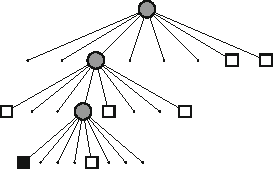
\includegraphics[scale=1.0]{octree_tree}
	}
	\hspace{5mm}
	\subfigure[Volumenstruktur]{
		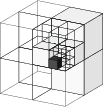
\includegraphics[scale=1.0]{octree_box}
	}
	\caption{Verfeinerung der \textit{octree} Darstellung durch Erfassung von besetzten (schwarz) und freien (weiß) Bereichen \cite{Hornung2013}. }
	\label{fig.octree}
	\end{center}
	%\vspace*{-8mm}
\end{figure}

Die Besonderheit des von Hornung \textit{et al.} entwickelten Ansatzes liegt darin, dass im Gegensatz zu einer binären Darstellung der Voxelzustände eine probabilistische Bewertung vorgenommen wird. Es können somit bei der Betrachtung der Voxel mehr als zwei Zustände unterschieden werden, so dass zwischen besetzten, freien und unbekannten Bereichen differenziert werden kann. Als Grenzwert der Verfeinerung kann eine anwendungsabhängige Auflösung definiert werden. Dabei ist auch die Kombination verschiedener Strukturbäume mit unterschiedlichen Auflösungen bei der Verwendung von \textit{Octomap} möglich, so dass bei Bedarf bestimmte Strukturen feiner aufgelöst werden können, um die Abbildungsgenauigkeit zu erhöhen.\\
Einen Vergleich zwischen Modellumgebung und der daraus erzeugten \textit{Octomap} zeigt \abb{fig.octomap}. Freie Voxel sind in der Abbildung nicht dargestellt, die Farbkodierung der Octomap bezieht sich daher auf die Höhenwerte der Modelldaten.\\

\begin{figure}[!ht]
	\begin{center}
	\subfigure[\textit{Octomap}]{
		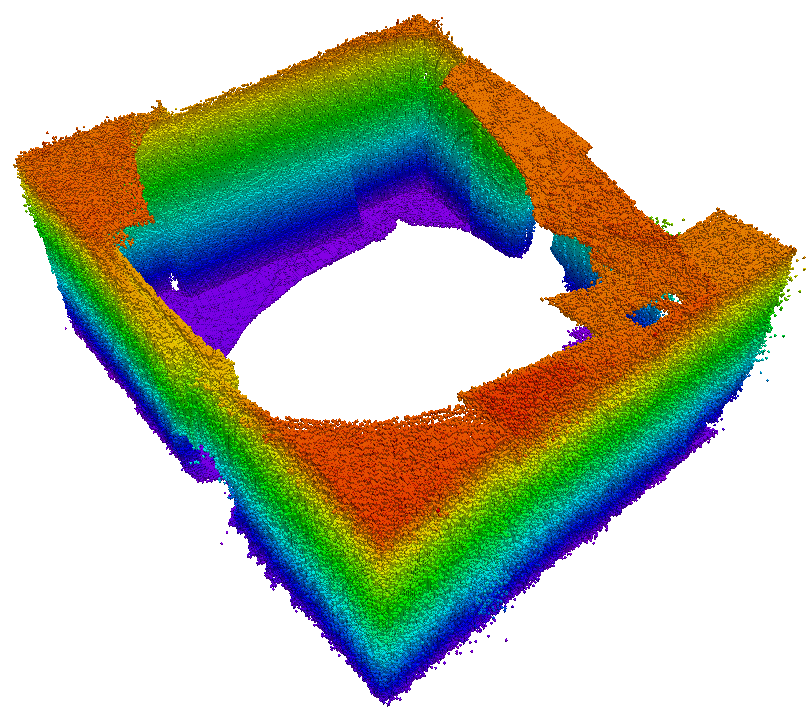
\includegraphics[scale=0.25]{octomap_rviz}
	}
	\hspace{5mm}
	\subfigure[Punktwolke]{
		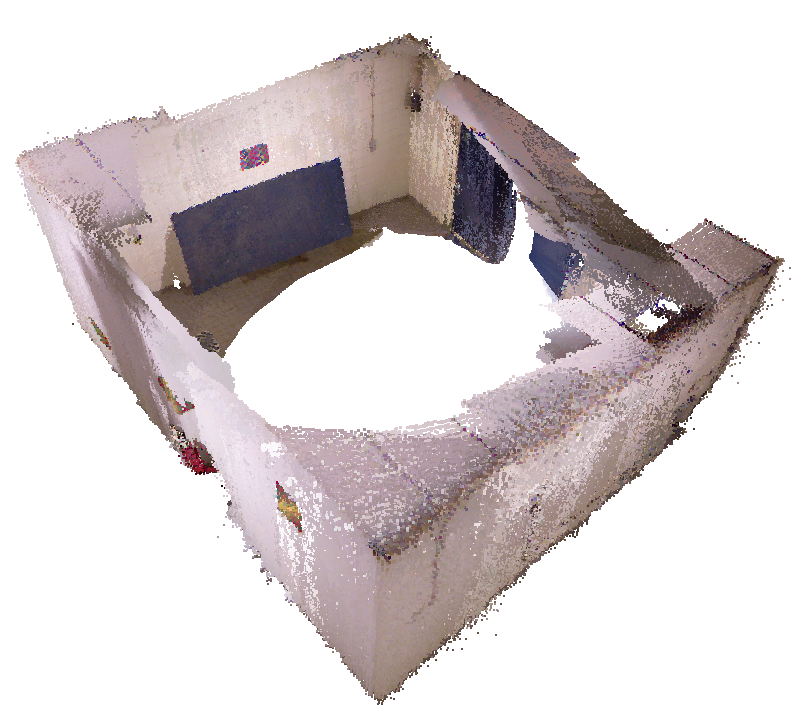
\includegraphics[scale=0.25]{pointcloud_meshlab}	
	}
	\caption{\textit{Octomap}-Struktur der Modellumgebung (a) abgeleitet aus der aufgezeichneten Punktwolke (b)}
	\label{fig.octomap}
	\end{center}
	%\vspace*{-8mm}
\end{figure}%

Ziel der Lokalisation ist die Bestimmung der Systempose innerhalb der Karte, also der Transformationsvorschrift zwischen den Koordinatensystemen des \kps{s} $\ks{KPS}$ und der Karte $\ks{M}$.\\
Die Transformation $\tmat{0}{M}$ ist konstant, da die Karte als statische Referenz bezüglich des globalen Koordinatensystems betrachtet werden kann. Die Lage kann somit beliebig gewählt werden, weshalb das Koordinatensystem im Folgenden in den globalen Ursprung gesetzt wird, so dass gilt:

\begin{equation}
\ks{0} = \ks{M}
\end{equation}

\section{Globale Lokalisation}
\label{chap.globloc}
Die globale Lokalisation dient zur Bestimmung der initialen Transformation des \kps{s} in der Karte. Es wird dafür zunächst ein Odometrie-Koordinatensystem $\ks{Odom}$ als Referenz eingeführt, dessen Lage im Rahmen der globalen Lokalisation ermittelte werden soll. Dieses Koordinatensystem stellt die Basis für die in der anschließenden lokalen Lokalisation zu bestimmende kontinuierliche Veränderung der Systempose dar.\\
Um die Abbildung zwischen \kps{} und Karte vollständig zu beschreiben wird außerdem die Transformation $\tmat{Odom}{KPS}$ definiert. Für die globale Lokalisation gilt dabei $\tmat{Odom}{KPS} = \vec{I}$, so dass die Koordinatensysteme $\ks{Odom}$ und $\ks{KPS}$ zusammenfallen.\\
Allgemein kann die Abbildung von Punkten im Koordinatensystem des \kps{s} ins Koordinatensystem der Karte für die globale Lokalisation damit beschrieben werden als:

\begin{equation}
\ve{M}{\tilde{P}} = \tmat{M}{Odom} \cdot \ve{KPS}{\tilde{P}}
\label{eq.globloc}
\end{equation}


Das in dieser Arbeit gewählte Verfahren zur globalen Lokalisation basiert auf dem \textit{Monte-Carlo-Algorithmus} \cite{Dellaert1999} und stellt damit wie in \abschnitt{chap:mcl} beschrieben einen partikelbasierten Ansatz dar.\\
Es wurde dazu eine Implementierung \cite{humanoidNavigation} verwendet, welche das Lokalisationsverfahren innerhalb einer ROS-Node bereitstellt. Als Referenz wird die zuvor beschriebene, aus der Modellumgebung erzeugte \textit{Octomap} verwendet.\\

\prever{
%\red[Entwickelt für die Lokalisation eines humanoiden Roboters konnte die Implementierung so angepasst werden, dass sie auch die Lokalisation eines handgeführten Systems ermöglicht.]\\
}

In der vorhandenen Umgebungskarte werden Partikel basierend auf einer Zufallsverteilung generiert. Jeder Partikel entspricht einer möglichen Pose des Kamera-Projektor-Systems und verfügt demnach über sechs Freiheitsgrade. Die Bestimmung der Pose des Kamera-Projektor-Systems erfolgt durch Auswertung der Partikel basierend auf einer Wahrscheinlichkeitsverteilung. Die Wahrscheinlichkeiten können dabei auf Basis zweier verschiedener Modelle berechnet werden, dem \textit{Endpoint}-Modell (EPM) und dem \textit{Raycasting}-Modell (RCM). Da sich beide Modelle bei der Berechnung der Wahrscheinlichkeiten auf die Log-Likelihood-Funktion stützen, soll diese zunächst kurz erläutert werden, bevor anschließend die beiden Modelle ausführlicher dargestellt werden.

\nomenclature[a]{EPM}{Endpoint-Modell}
\nomenclature[a]{RCM}{Raycasting-Modell}

\subsection{Log-Likelihood-Funktion}
\label{chap.loglik}
Ideale Entfernungsmesser würden bei einer Messung die exakten Distanzen zu den Hindernissen in ihrem Messbereich ermitteln. In der Realität sind jedoch alle Messungen mit einem Fehler durch lokales Messrauschen behaftet, welches im Fall der Kinect als Gaußverteilung modelliert werden kann \cite{Nguyen2012}.\\

Es soll dazu die Pose $\vec{x}_{\ind{p}}$ eines Partikels innerhalb der Karte $m$ betrachtet. Die Wahrscheinlichkeit $p$, ob eine gemessene Distanz $d_{\ind{m}}^i$ aus einem bekannten Hindernis in der Entfernung $d_{\ind{k}}$ resultiert, lässt sich somit innerhalb des Intervalls der Sensorreichweite $[d_{\ind{min}};d_{\ind{max}}]$ über eine Gaußverteilung mit Mittelwert $d_{\ind{k}}$ und der Varianz des Sensors $\sigma_{\ind{S}}^2$ ermitteln \cite{Thrun2005}:

\begin{equation}
p(d_\ind{m}^i|\vec{x}_{\ind{p}},m) = \left\lbrace\begin{array}{ll}
\eta  \cdot \mathcal{N}(d_{\ind{m}}^i;d_{\ind{k}},\sigma_{\ind{S}}^2) & \quad \mathrm{wenn} \quad d_{\ind{min}}\leq d_{\ind{m}}^i \leq d_{\ind{max}} \\
0 & \quad \mathrm{sonst}
\end{array}
\right.
\end{equation}

\nomenclature[l]{$\vec{x}_{\ind{p}}$}{Pose eines Partikels}
\nomenclature[l]{$m$}{Karte}
\nomenclature[l]{$p$}{Wahrscheinlichkeitswert eines Partikels}
\nomenclature[l]{$d_{\ind{m}}^i$}{i-ter Wert einer Entfernungsmessung}
\nomenclature[l]{$d_{\ind{k}}$}{Distanzwert eines Hindernisses}
\nomenclature[l]{$d_{\ind{min}}$}{Minimal auflösbare Sensordistanz}
\nomenclature[l]{$d_{\ind{max}}$}{Maximal auflösbare Sensordistanz}
\nomenclature[g]{$\sigma_{\ind{S}}$}{Standardabweichung des Sensors}
\nomenclature[g]{$\eta$}{Normalisierungsfaktor}
\nomenclature[l]{$\vec{d}_{\ind{m}}$}{Vektor aus Messwerten einer Messung}
\nomenclature[l]{$\Delta d$}{Differenz aus Messwert und Distanzwert der Karte}
\nomenclature[l]{$\mathrm{K}$}{Konstante}

Dabei ist $\eta$ ein für die verwendeten Modelle konstanter Normalisierungsfaktor und die Gaußverteilung mit der Differenz der Distanzen $\Delta d = d_{\ind{m}}^i-d_{\ind{k}}$  gegeben durch:

\begin{equation}
\mathcal{N}(d_{\ind{m}}^i;d_{\ind{k}},\sigma_{\ind{S}}^2) = \frac{1}{\sqrt{2 \cdot \pi \cdot \sigma_{\ind{S}}^2}}  \cdot e^{-\dfrac{1}{2} \cdot \dfrac{{(\Delta d})^2}{\sigma_{\ind{S}}^2}}
\end{equation}

Die Bestimmung der Wahrscheinlichkeit einer Pose erfolgt durch Betrachtung aller $n$, im Vektor $\vec{d}_{\ind{m}}$ zusammengefassten, Messwerte. Dazu wird angenommen, dass die Messwerte voneinander unabhängig sind und das Produkt der einzelnen Wahrscheinlichkeiten gebildet \cite{Hornung2010}. Dies ergibt die Likelihood-Funktion:

\begin{equation}
\label{eq.likelihood}
p(\vec{d}_{\ind{m}}|\vec{x}_{\ind{p}},m) = \prod_{i=1}^{n}p(d_{\ind{m}}^i|\vec{x}_{\ind{p}},m)
\end{equation}

Durch Anwendung des natürlichen Logarithmus auf \eq{eq.likelihood} ergibt sich die Log-Likelihood-Funktion und die Berechnung vereinfacht sich zur Bildung der Summe über die Messwerte:

\begin{equation}
\begin{split}
\log \: p(\vec{d}_{\ind{m}}|\vec{x}_{\ind{p}},m) & = \sum_{i=1}^{n}\log\: p(d_{\ind{m}}^i|\vec{x}_{\ind{p}},m) \\[1em]
& = \sum_{i=1}^{n}\log \left( \frac{1}{\sqrt{2 \cdot \pi \cdot \sigma_{\ind{S}}^2}} \cdot e^{-\dfrac{1}{2} \cdot \dfrac{{(\Delta d})^2}{\sigma_{\ind{S}}^2}} \right)\\[1em]
& = \underbrace{-\frac{1}{2} \cdot \log(2 \cdot \pi \cdot\sigma_{\ind{S}}^2)}_{\ind{K}}-\dfrac{\sum_{i=1}^{n}(\Delta d)^2}{2 \cdot \sigma_{\ind{S}}^2}
\end{split}
\end{equation}
Da der natürliche Logarithmus eine streng monotone Funktion ist, bleibt die Stelle des Maximums der Ursprungsfunktion erhalten. Das bedeutet, dass der Partikel mit maximalem Wahrscheinlichkeitswert erhalten bleibt. Da die Partikel bei jeder Lokalisation lediglich relativ untereinander verglichen werden, hat dieser Schritt keine Auswirkungen auf das Ergebnis. Die Konstante $\mathrm{K}$ ist bei gleichbleibender Varianz für alle Messungen identisch und kann daher vorab berechnet werden.\\
Die so bestimmte Wahrscheinlichkeit der betrachteten Pose kann nun als Gewichtung verwendet werden, um das Maximum über alle Partikel zu bestimmen. 

\subsection{Endpoint-Modell}
Das EPM, welches von Konolige und Chou in \cite{Konolige1999} beschrieben wurde, bestimmt die Wahrscheinlichkeit einer Pose anhand eines Distanz-Modells. Basierend auf der für die Lokalisation verwendeten \textit{Octomap} wird zunächst eine Lookup-Table erstellt, welche die räumlichen Dimensionen der Ausgangskarte abbildet. Jedem Voxel wird dabei basierend auf der Entfernung zum nächsten Hindernis ein Distanzwert zugewiesen. Als Hindernisse gelten alle besetzten Zellen der \textit{Octomap}, also neben dem Raum selbst auch alle weiteren in der Karte vorhanden Strukturen. Bei der Bestimmung der Distanzwerte werden die Messunsicherheiten des verwendeten Sensors berücksichtigt, so dass ein Abbild der Karte wie in \abb{fig.dist_map} erzeugt wird.

\begin{figure}[!ht]
	\begin{center}
	
	\subfigure[Original-Karte]{
		\begingroup\fboxsep=0pt\fboxrule=1pt
		\fbox{%
			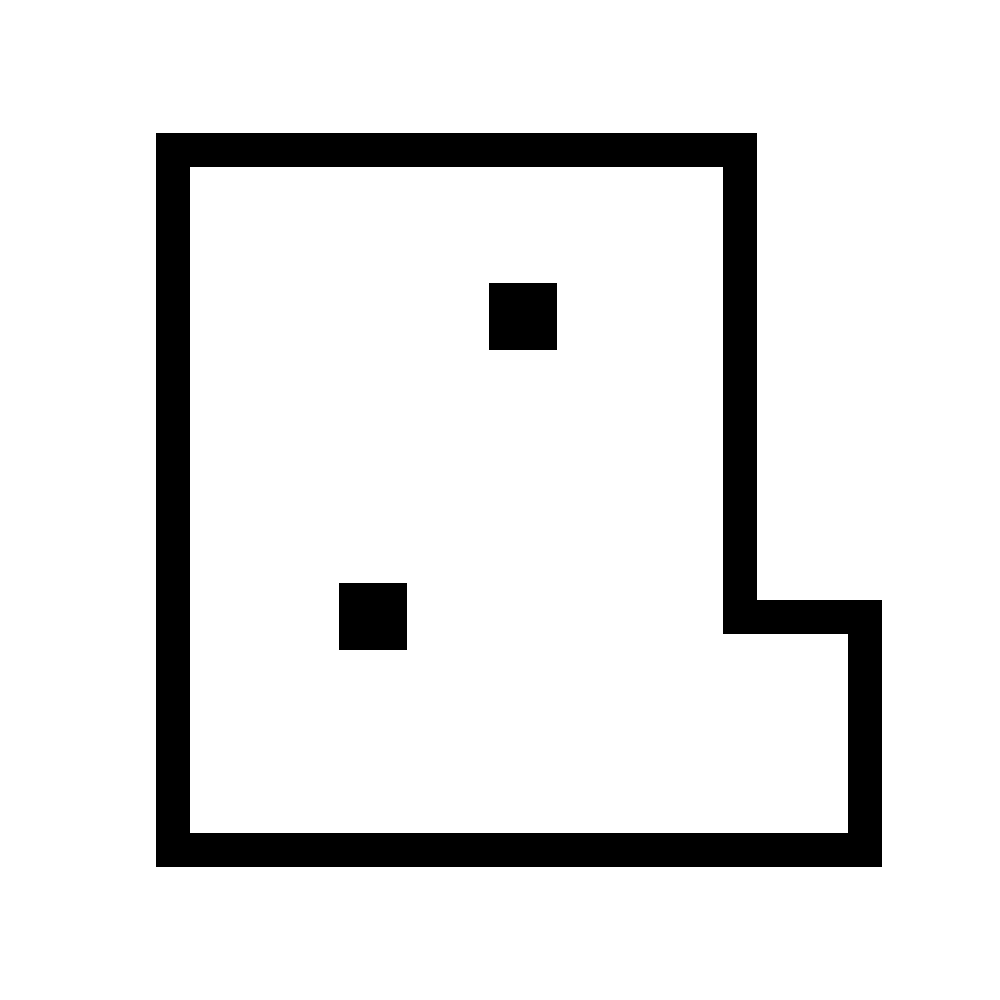
\includegraphics[scale=0.25]{distance_map_orig}%
		}
		\endgroup
	}
	\hspace{5mm}
	\subfigure[Distanz-Karte]{
		\begingroup\fboxsep=-1pt\fboxrule=2pt
		\fbox{%
			
\includegraphics[scale=0.25]{distance_map}%	
		}
		\endgroup
	}
	\caption{Abbildung der Karte (a) als Distanz-Modell (b)}
	\label{fig.dist_map}
	\end{center}
	%\vspace*{-8mm}
\end{figure}

Erfolgt die Lokalisation wie in dieser Arbeit innerhalb einer statischen Umgebung kann die Berechnung der Distanz-Karte bereits vor der Lokalisation erfolgen. In jedem Schritt der Lokalisation kann dadurch eine deutliche Verringerung des Rechenaufwands erzielt werden. Anzumerken bleibt, dass die Distanz-Karte während der gesamten Programmlaufdauer im Speicher behalten wird und bezüglich des Speicherbedarfs die Ausgangskarte deutlich übersteigen kann.\\

Die Lokalisation erfolgt beim EPM indem die durch die Kinect aufgenommene Punktwolke betrachtet wird. Die Einträge werden als Endpunkte der Strahlen interpretiert, welche von der Kamera an der jeweiligen Partikelpose ausgesendet werden. Durch Abbildung auf die zuvor berechnete Distanz-Karte können die darin gespeicherten Werte für $\Delta d$ ausgelesen werden. Die Wahrscheinlichkeit, dass die Punktwolke von der Stelle des betrachteten Partikels aus aufgenommen wurde, lässt sich anschließend anhand der Distanzwerte bestimmen. Die berechneten Wahrscheinlichkeiten aller Strahlen werden innerhalb der unter \abschnitt{chap.loglik} beschriebenen Log-Likelihood-Funktion addiert, um den Partikel mit der höchsten Gewichtung zu ermitteln.\\

Das EPM bildet durch den verwendeten Ansatz nicht direkt die physikalische Arbeitsweise eines Entfernungsmessers ab, da es durch Hindernisse \glqq hindurchsehen\grqq{} kann, wie \abb{fig.endpoint} zeigt. Die Sensorstrahlen durchqueren Bereiche, welche als Hindernisse in der Distanz-Karte eingetragen sind. Das EPM registriert dies jedoch nicht, da lediglich die Endpunkte der Strahlen betrachtet werden. Obwohl so eventuell unmögliche Posen ermittelt werden können, ist das EPM generell in der Lage, eine zuverlässige Approximation der wahren Systempose zu bestimmen \cite{Konolige1999}.\\

%\red[An welcher Stelle?: Die Bestimmung erfolgt mittels der Log-Likelihood-Funktion, welche eine statistische Aussage über die Wahrscheinlichkeit der Messung berechnet.\\]

\begin{figure}[!ht]
	\begin{center}
		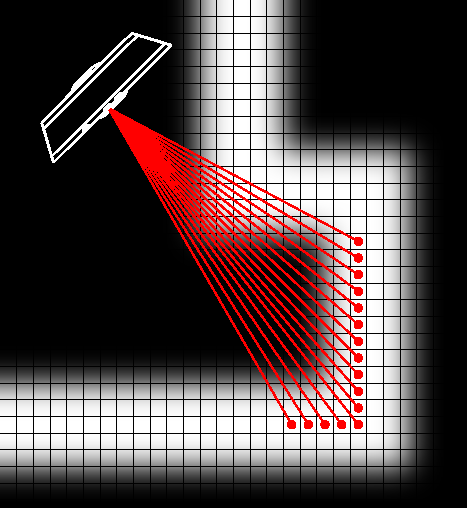
\includegraphics[scale=1.0]{endpoint_from_dist}
		\caption{Mögliche Fehllokalisation des \textit{Endpoint}-Modells}
		\label{fig.endpoint}
	\end{center}
	%\vspace*{-8mm}
\end{figure}

\subsection{Raycasting-Modell}
Beim RCM, beschrieben von Thrun \textit{et al.} in \cite{Thrun2005}, werden für jede Pose nicht die Endpunkte der ausgesendeten Strahlen betrachtet, sondern ihr Verlauf. Entlang der Strahlen von der Kamera zu den Messpunkten der aufgenommenen Punktwolke findet ein Abgleich mit den Daten der Karte statt. Erreicht der Strahl einen besetzen Bereich in der Karte endet die Betrachtung wie in \abb{fig.raycast} dargestellt. Freie Bereiche sind in der Darstellung grün und besetzte Bereiche rot gekennzeichnet.

\begin{figure}[!ht]
	\begin{center}
		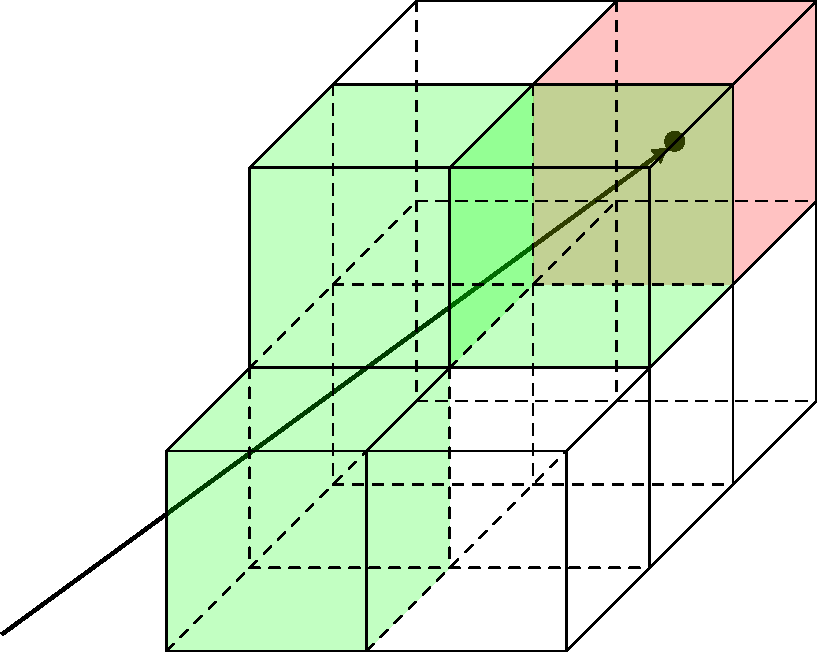
\includegraphics[scale=0.5]{raycasting}
		\caption{Betrachtung des Strahlenverlaufs beim \textit{Raycasting}-Modell}
		\label{fig.raycast}
	\end{center}
	%\vspace*{-8mm}
\end{figure}

\prever{
\red[isometrisch besser?\\]
}
Die Entfernung zwischen dem ermittelten Punkt und dem betrachteten Partikel wird anschließend berechnet und mit der Entfernung des zugehörigen Sensorwertes verglichen. Die Differenz $\Delta d$ der beiden Distanzen wird verwendet, um die Wahrscheinlichkeit zu bestimmen, dass der Sensorwert an dieser Stelle aufgenommen wurde. Die Berechnung der jeweiligen Wahrscheinlichkeit erfolgt beim RCM wie auch beim EPM mittels der Log-Likelihood-Funktion.\\

Als zusätzliches Bewertungsmaß der globalen Lokalisation wurde die Berechnung des Quadratischen Mittels der Distanzen implementiert. Die Ergebnisse korrelieren aufgrund der unterschiedlichen Berechnungsweisen nicht exakt mit den ermittelten Wahrscheinlichkeitswerten, erlauben jedoch eine Bewertung der Überdeckung zwischen Karten- und Sensordaten. Im Gegensatz zu den absoluten Gewichten der Partikel bietet dieses Maß damit eine Möglichkeit Lokalisationen mit unterschiedlichen Modellparametern zu vergleichen.

\prever{
%\red[Markerbasierte Lokalisation\\]
%\red["Tracking" durch Verringerung der Partikelanzahl möglich, da sich die Rechenzeit deutlich verringert]\\
}

\section{Lokale Lokalisation}
\label{locloc}
Im Anschluss an die globale Lokalisation wird die Bewegung des Systems kontinuierlich verfolgt und die aktuelle Pose aktualisiert. Das Tracking dient damit der Bestimmung der Transformation $\tmat{Odom}{KPS}$, welche die Abbildung zwischen den Koordinaten des \kps{s} und der Karte beschreibt und während der globalen Lokalisation als Einheitsmatrix definiert wurde.\\

Da das handgeführte System nicht über Odometriedaten verfügt, wie sie beispielsweise bei einem mobilen Robotersystem durch Messungen der Radumdrehungen zur Verfügung stehen, muss das Tracking auf Basis anderer Sensordaten durchgeführt werden. Dazu wird die in \abschnitt{chap.unimod} beschriebene visuelle Odometrie eingesetzt und eine Fusion mit den Daten der inertialen Messeinheit durchgeführt.\\

\prever{
\subsection{Visuelle Odometrie}
}
Die visuelle Odometrie basiert auf den Bilddaten der Kinect. Neben dem Farbbild wird wie in \abb{fig.fovis} (a) auch die aus dem Infrarotbild bestimmte Tiefenkarte ausgewertet. Dabei wird eine Implementierung \cite{Fovis} eingesetzt, welche die visuelle Odometrie als quelloffene Bibliothek für ROS bereitstellt.\\
Die Bestimmung der visuellen Odometrie erfolgt dabei in sechs aufeinanderfolgenden Schritten \cite{Huang2011}:

\begin{enumerate}
\item Das Farbbild wird in ein Grauwertbild konvertiert und mittels eines Gauß-Kernels geglättet. Es wird außerdem eine Gauß-Pyramide\footnote{Eine Gauß-Pyramide ist eine Sammlung von Bildern, welche ausgehend vom Originalbild durch Tiefpassfilterung und anschließende Verkleinerung der Bilder um den Faktor $\nicefrac{1}{4}$ aufgebaut wird. Sie ermöglicht die effiziente Erkennung relevanter Bildmerkmale, da die Bildanalyse in der obersten Ebene begonnen werden kann und nur bei Bedarf die tiefer liegende, höher aufgelöste Ebene betrachtet wird \cite{Nischwitz20112}.} angelegt, um eine robustere Detektion der Bildmerkmale zu ermöglichen.
\item Innerhalb jeder Ebene der Gauß-Pyramide wird eine Merkmalserkennung mit adaptivem Schwellwert durchgeführt. Alle Merkmale ohne korrespondierende Informationen innerhalb des Tiefenbildes werden an dieser Stelle verworfen.
\item Anhand des aktuellen und des vorangegangenen Bildes wird eine initiale Approximation der Rotation des Systems durchgeführt, um den Suchbereich für anschließende Merkmalsextraktionen eingrenzen zu können.\\
An dieser Stelle ist anzumerken, dass diese Methode für den Anwendungsfall eines autonomen, fliegenden Systems ausgelegt ist. Da ein handgeführtes System jedoch die gleichen Freiheitsgrade besitzt, kann das Verfahren ohne Einschränkungen genutzt werden.
\item Den extrahierten Merkmalen wird ein Deskriptor zugewiesen, welcher einen Vergleich der Merkmale in aufeinander folgenden Bildern ermöglicht. Durch Minimierung der Fehlerquadrate der einander zugeordneten Deskriptoren kann anschließend die Lokalisation des Merkmals verfeinert und somit ein Abgleich im sub-pixel Bereich durchgeführt werden.
\item Um die Plausibilität zu überprüfen und falsch erkannte Merkmale zu eliminieren wird ein Vergleich der Merkmale zwischen den Bildern durchgeführt. Ausgehend von der Annahme, dass es sich um eine statische Szene handelt, kann dazu die euklidische Distanz zwischen den Positionen der Merkmale verwendet werden.
\item Für die finale Bestimmung der Odometrie des Systems wird zunächst die Transformation zwischen den Posen der aufgenommenen Bilder durch Minimierung der euklidischen Distanzen zwischen den verbliebenen Merkmalen bestimmt. Durch Minimierung des Rückprojektionsfehlers wird diese Transformation anschließend verfeinert. Eine weitere Verfeinerung wird erreicht, indem Merkmale mit zu großem Fehler in der Rückprojektion aus der Betrachtung entfernt werden.
\end{enumerate}
Die visuelle Odometrie liefert durch das beschrieben Verfahren ein Ergebnis für die Veränderung der aktuellen Pose bezüglich aller sechs Freiheitsgrade. \abb{fig.fovis} (b) zeigt die aus zwei aufeinander folgenden Bildern ermittelte Veränderung der Pose anhand der Merkmale.\\

\begin{figure}[!ht]
	\begin{center}
	\subfigure[RGB-Kamerabild (oben) und zugehörige Tiefenwerte (unten)]{
		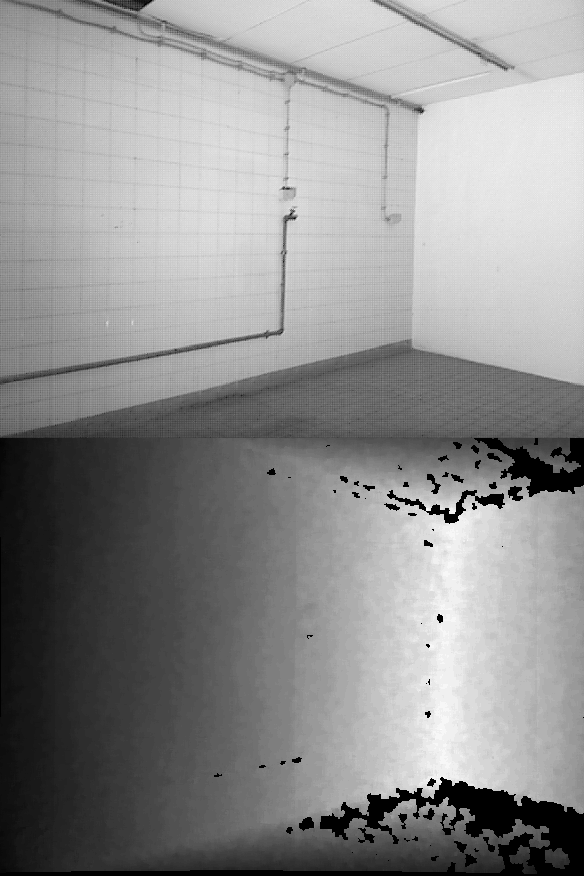
\includegraphics[width=5cm]{fovis_combined}
	}
	\hspace{5mm}
	\subfigure[Abgleich der Bildmerkmale in aufeinander folgenden Kamerabildern]{
		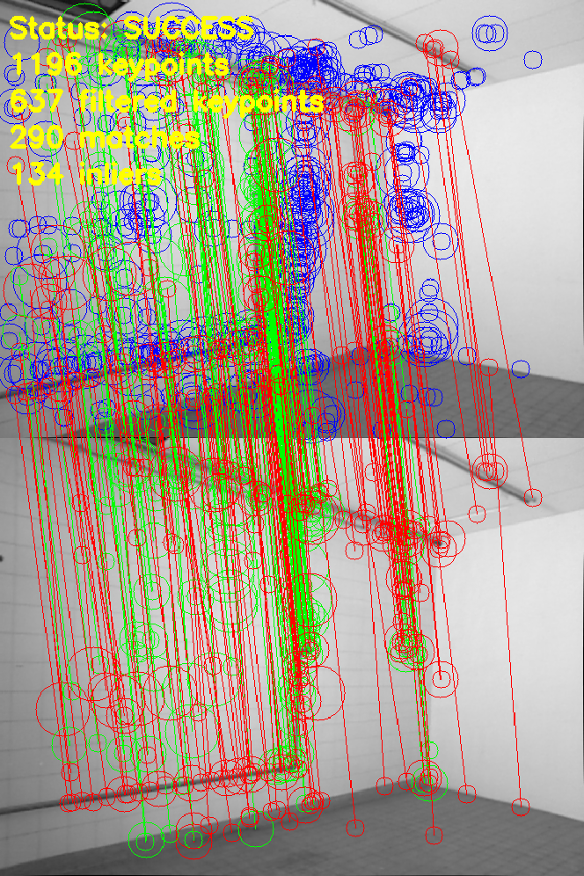
\includegraphics[width=5cm]{fovis_features}
	}
	\caption{Bestimmung der visuellen Odometrie aus RGB- und Tiefenbild}
	\label{fig.fovis}
	\end{center}
	%\vspace*{-8mm}
\end{figure}

Die Pose des \kps{s} wird im Rahmen der lokalen Lokalisation mit Bezug auf das Referenz-Koordinatensystem $\ks{Odom}$ bestimmt. Die in \eq{eq.globloc} aufgeführte Abbildungsgleichung wird damit unter Berücksichtigung der ermittelten Transformation $\tmat{Odom}{KPS}$ erweitert zu:

\begin{equation}
\ve{M}{\tilde{P}} = \tmat{M}{Odom} \cdot \tmat{Odom}{KPS} \cdot \ve{KPS}{\tilde{P}}
\label{eq.locloc}
\end{equation}

\prever{
%\red[Um eine höhere Genauigkeit zu erreichen werden ergänzend die Messdaten einer inertialen Messeinheit betrachtet.\\]
%\red[IMU eigentlich in beiden Verfahren eingesetzt!?]
}
\prever{
%\subsection{Inertiale Messeinheit}
}
\section{Inertiale Messeinheit}
Die in \abschnitt{chap.imu} beschriebene inertiale Messeinheit ist in der Lage die translatorischen und rotatorischen Beschleunigungen des Systems zu messen. Auf Basis des von Mahony \textit{et al.} \cite{Mahony2008} entwickelten Algorithmus wird aus den Messdaten die Orientierung der Messeinheit bestimmt. Die verwendete Implementierung für den Arduino Nano (\abschnitt{chap.arduino}) zur Anbindung an das System basiert auf \cite{IMUCode}.\\
Um die Messdaten in die Programmstruktur einzubinden wurde die Implementierung um eine Schnittstelle für ROS erweitert. Darüber hinaus wurde eine Gravitationskompensation implementiert, welche neben der Bestimmung des Roll- und Nick-Winkels des \kps{s} auch das Auslesen der relativen Beschleunigungen des Systems ermöglicht.\\

Die globale Lokalisation verwendet die bestimmten Winkel bezüglich der Roll- und Nick-Achse in der Initialisierung der Partikel. Es können dadurch zwei Freiheitsgrade der Pose direkt bestimmt werden, wodurch der erforderliche Rechenaufwand deutlich reduziert werden kann.\\

Als Ergänzung der visuellen Odometrie werden die Messdaten der inertialen Messeinheit mit den Odometriedaten fusioniert. Dabei werden sowohl die Werte des Roll- und Nick-Winkels als auch die ermittelten Beschleunigungswerte entlang der Koordinatenachsen des \kps{s} berücksichtigt. Die Fusion der Sensordaten wird durch ein Erweitertes-Kalman-Filter realisiert.

\prever{
%\subsection{Erweitertes Kalman-Filter}
}
\section{Erweitertes Kalman-Filter}
\label{chap.kalman}
Das Kalman-Filter \cite{Kalman1960} stellt eine in der Praxis bewährte Methode zur Fusion von Sensordaten dar. Es ermöglicht die Vorhersage des aktuellen Systemzustands durch statistische Approximation. Der Ausgang jeder auf ein System wirkenden Aktion, beispielsweise die Drehung der Räder, kann in der Realität nicht ohne Unsicherheiten vorhergesagt werden. Der neue Systemzustand ist deshalb allein auf Basis der Odometriedaten nur mit großer Varianz bestimmbar. Messungen können dazu verwendet werden, diese Unsicherheiten zu korrigieren, um den realen Zustand mit höherer Genauigkeit schätzen zu können.\\

Die Besonderheit des Kalman-Filters liegt darin, dass die Unsicherheiten der Messungen und Aktionsresultate durch Gaußverteilungen mit dem Erwartungswert $\mu$ und der Standardabweichung $\sigma$ modelliert werden \cite{Hertzberg2012}.\\
Durch das Erweiterte Kalman-Filter (EKF) kann das Filterprinzip mittels Linearisierung der Systemzustände auch auf nichtlineare Systeme angewendet werden. In dieser Arbeit wurde eine Implementierung des EKF verwendet \cite{EKF}, welche eine direkte Anbindung an ROS zur Verfügung stellt. Die auf das handgeführte System einwirkenden Aktionen, insbesondere also die Bewegung des Systems durch den Anwender, werden dabei durch die verwendete visuelle Odometrie detektiert.\\
Mit Hilfe der inertialen Messeinheit kann die bestimmte Systempose aktualisiert und verfeinert werden. Dabei werden neben den absoluten Werten des Roll- und Nick-Winkels auch die Beschleunigungen bezüglich der drei Systemachsen integriert, um die Bewegung des Systems zu schätzen. \abb{fig.kalman} zeigt
exemplarisch das Prinzip der Zustandsannäherung durch die visuelle Odometrie ($\mu_O$, $\sigma_O$) und die auf Basis der Messwerte der IMU ($\mu_I$, $\sigma_I$) durchgeführte Korrektur.
\prever{
\red[in anlehung an Hertzberg s.134]
}%
\prever{
\red[verschieben nach Stand der Technik?]\red[Beschreibung!]\\
}
\begin{figure}[ht]
	\begin{center}%
		\includesvgnew[1]{images/kalman}%
%		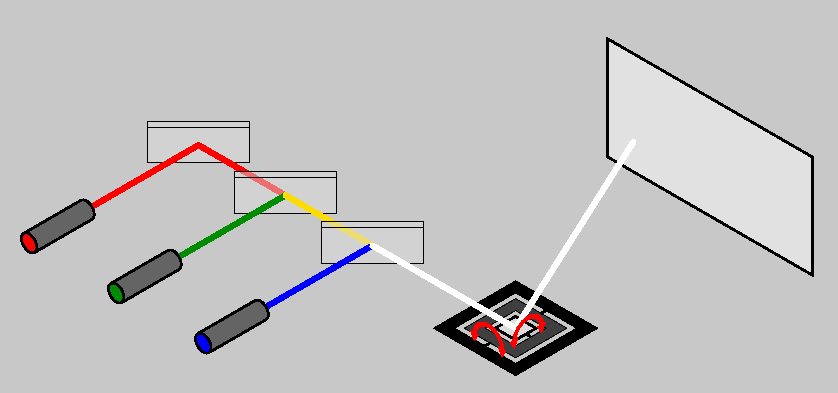
\includegraphics[scale=1.0]{projector_tech_02}
		\caption{Approximation des Systemzustands durch das Kalman-Filter. Darstellung nach \cite{Hertzberg2012}}
		\label{fig.kalman}
	\end{center}
	\vspace*{-8mm}
\end{figure}

\prever{
\red[plot?\\
Darstellung überarbeiten! Indizes korrekt!?\\]
}

\nomenclature[g]{$\mu_{\ind{O}}$}{Mittelwert einer Messung auf Basis der visuellen Odometrie}
\nomenclature[g]{$\mu_{\ind{I}}$}{Mittelwert einer Messung auf Basis der IMU}
\nomenclature[g]{$\sigma_{\ind{O}}$}{Standardabweichung einer Messung auf Basis der visuellen Odometrie}
\nomenclature[g]{$\sigma_{\ind{I}}$}{Standardabweichung einer Messung auf Basis der IMU}
\nomenclature[g]{$\mu_{\ind{EKF}}$}{Durch das EKF angenäherter Mittelwert}
\nomenclature[g]{$\sigma_{\ind{EKF}}$}{Durch das EKF angenäherte Standardabweichung}


\nomenclature[a]{EKF}{Erweitertes Kalman-Filter}

%\red[Ergebnis der Lokalisation in Darstellung zusammenfassen? EKF kombiniert Messwerte und liefert $\tmat{Odom}{K}$, globale Lokalisatoin liefert $\tmat{M}{Odom}$, kombiniert ergibt sich $\tmat{M}{K}$\\]


\prever{
\begin{figure}[!ht]
	\begin{center}
		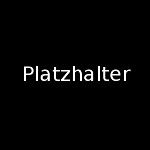
\includegraphics[scale=1.0]{spacer}
		\caption{EKF Übersicht - Kombination der Messwerte und ausgegebene Transformation}
		\label{fig.ekf}
	\end{center}
	%\vspace*{-8mm}
\end{figure}

\red[Ergebnis der Lokalisation in Darstellung zusammenfassen? EKF kombiniert Messwerte und liefert $\tmat{Odom}{K}$, globale Lokalisatoin liefert $\tmat{M}{Odom}$, kombiniert ergibt sich $\tmat{M}{K}$\\]

%\red[%odometrie auch Messung...Varianz der -sensoren aber klein gegenüber dem Umgebungseinfluss]
%Partikelbasiertes Tracking\\
%Featurebasiertes Tracking\\
%Beschleunigungsdatenbasiertes Tracking\\
%Kombination der Odometriedaten durch Extended Kalman Filter \red[Buch Hertzberg]\\
%\red[Ergebnisse der Kalman Einbindung mit und ohne IMU auswerten]
%\red[Fovis differential auf true und imu auf false?]
}